% GNUPLOT: LaTeX picture with Postscript
\begingroup
  \makeatletter
  \providecommand\color[2][]{%
    \GenericError{(gnuplot) \space\space\space\@spaces}{%
      Package color not loaded in conjunction with
      terminal option `colourtext'%
    }{See the gnuplot documentation for explanation.%
    }{Either use 'blacktext' in gnuplot or load the package
      color.sty in LaTeX.}%
    \renewcommand\color[2][]{}%
  }%
  \providecommand\includegraphics[2][]{%
    \GenericError{(gnuplot) \space\space\space\@spaces}{%
      Package graphicx or graphics not loaded%
    }{See the gnuplot documentation for explanation.%
    }{The gnuplot epslatex terminal needs graphicx.sty or graphics.sty.}%
    \renewcommand\includegraphics[2][]{}%
  }%
  \providecommand\rotatebox[2]{#2}%
  \@ifundefined{ifGPcolor}{%
    \newif\ifGPcolor
    \GPcolorfalse
  }{}%
  \@ifundefined{ifGPblacktext}{%
    \newif\ifGPblacktext
    \GPblacktexttrue
  }{}%
  % define a \g@addto@macro without @ in the name:
  \let\gplgaddtomacro\g@addto@macro
  % define empty templates for all commands taking text:
  \gdef\gplbacktext{}%
  \gdef\gplfronttext{}%
  \makeatother
  \ifGPblacktext
    % no textcolor at all
    \def\colorrgb#1{}%
    \def\colorgray#1{}%
  \else
    % gray or color?
    \ifGPcolor
      \def\colorrgb#1{\color[rgb]{#1}}%
      \def\colorgray#1{\color[gray]{#1}}%
      \expandafter\def\csname LTw\endcsname{\color{white}}%
      \expandafter\def\csname LTb\endcsname{\color{black}}%
      \expandafter\def\csname LTa\endcsname{\color{black}}%
      \expandafter\def\csname LT0\endcsname{\color[rgb]{1,0,0}}%
      \expandafter\def\csname LT1\endcsname{\color[rgb]{0,1,0}}%
      \expandafter\def\csname LT2\endcsname{\color[rgb]{0,0,1}}%
      \expandafter\def\csname LT3\endcsname{\color[rgb]{1,0,1}}%
      \expandafter\def\csname LT4\endcsname{\color[rgb]{0,1,1}}%
      \expandafter\def\csname LT5\endcsname{\color[rgb]{1,1,0}}%
      \expandafter\def\csname LT6\endcsname{\color[rgb]{0,0,0}}%
      \expandafter\def\csname LT7\endcsname{\color[rgb]{1,0.3,0}}%
      \expandafter\def\csname LT8\endcsname{\color[rgb]{0.5,0.5,0.5}}%
    \else
      % gray
      \def\colorrgb#1{\color{black}}%
      \def\colorgray#1{\color[gray]{#1}}%
      \expandafter\def\csname LTw\endcsname{\color{white}}%
      \expandafter\def\csname LTb\endcsname{\color{black}}%
      \expandafter\def\csname LTa\endcsname{\color{black}}%
      \expandafter\def\csname LT0\endcsname{\color{black}}%
      \expandafter\def\csname LT1\endcsname{\color{black}}%
      \expandafter\def\csname LT2\endcsname{\color{black}}%
      \expandafter\def\csname LT3\endcsname{\color{black}}%
      \expandafter\def\csname LT4\endcsname{\color{black}}%
      \expandafter\def\csname LT5\endcsname{\color{black}}%
      \expandafter\def\csname LT6\endcsname{\color{black}}%
      \expandafter\def\csname LT7\endcsname{\color{black}}%
      \expandafter\def\csname LT8\endcsname{\color{black}}%
    \fi
  \fi
    \setlength{\unitlength}{0.0500bp}%
    \ifx\gptboxheight\undefined%
      \newlength{\gptboxheight}%
      \newlength{\gptboxwidth}%
      \newsavebox{\gptboxtext}%
    \fi%
    \setlength{\fboxrule}{0.5pt}%
    \setlength{\fboxsep}{1pt}%
\begin{picture}(10080.00,2880.00)%
    \gplgaddtomacro\gplbacktext{%
      \csname LTb\endcsname%%
      \put(876,469){\makebox(0,0)[r]{\strut{}-0.6}}%
      \csname LTb\endcsname%%
      \put(876,831){\makebox(0,0)[r]{\strut{}-0.4}}%
      \csname LTb\endcsname%%
      \put(876,1193){\makebox(0,0)[r]{\strut{}-0.2}}%
      \csname LTb\endcsname%%
      \put(876,1555){\makebox(0,0)[r]{\strut{}0.0}}%
      \csname LTb\endcsname%%
      \put(876,1916){\makebox(0,0)[r]{\strut{}0.2}}%
      \csname LTb\endcsname%%
      \put(876,2278){\makebox(0,0)[r]{\strut{}0.4}}%
      \csname LTb\endcsname%%
      \put(876,2640){\makebox(0,0)[r]{\strut{}0.6}}%
      \csname LTb\endcsname%%
      \put(1378,68){\makebox(0,0){\strut{}$0.0$}}%
      \csname LTb\endcsname%%
      \put(1747,68){\makebox(0,0){\strut{}$0.4$}}%
      \csname LTb\endcsname%%
      \put(2117,68){\makebox(0,0){\strut{}$0.8$}}%
      \csname LTb\endcsname%%
      \put(2486,68){\makebox(0,0){\strut{}$1.2$}}%
      \csname LTb\endcsname%%
      \put(2856,68){\makebox(0,0){\strut{}$1.6$}}%
    }%
    \gplgaddtomacro\gplfronttext{%
      \csname LTb\endcsname%%
      \put(238,1554){\rotatebox{-270}{\makebox(0,0){\strut{}$\psi_{\rm central}$}}}%
    }%
    \gplgaddtomacro\gplbacktext{%
      \csname LTb\endcsname%%
      \put(3093,469){\makebox(0,0)[r]{\strut{}}}%
      \csname LTb\endcsname%%
      \put(3093,831){\makebox(0,0)[r]{\strut{}}}%
      \csname LTb\endcsname%%
      \put(3093,1193){\makebox(0,0)[r]{\strut{}}}%
      \csname LTb\endcsname%%
      \put(3093,1555){\makebox(0,0)[r]{\strut{}}}%
      \csname LTb\endcsname%%
      \put(3093,1916){\makebox(0,0)[r]{\strut{}}}%
      \csname LTb\endcsname%%
      \put(3093,2278){\makebox(0,0)[r]{\strut{}}}%
      \csname LTb\endcsname%%
      \put(3093,2640){\makebox(0,0)[r]{\strut{}}}%
      \csname LTb\endcsname%%
      \put(3595,68){\makebox(0,0){\strut{}$0.0$}}%
      \csname LTb\endcsname%%
      \put(3964,68){\makebox(0,0){\strut{}$0.3$}}%
      \csname LTb\endcsname%%
      \put(4334,68){\makebox(0,0){\strut{}$0.6$}}%
      \csname LTb\endcsname%%
      \put(4703,68){\makebox(0,0){\strut{}$0.9$}}%
      \csname LTb\endcsname%%
      \put(5073,68){\makebox(0,0){\strut{}$1.2$}}%
    }%
    \gplgaddtomacro\gplfronttext{%
      \csname LTb\endcsname%%
      \put(5455,-262){\makebox(0,0){\strut{}$\tau$}}%
    }%
    \gplgaddtomacro\gplbacktext{%
      \csname LTb\endcsname%%
      \put(5311,469){\makebox(0,0)[r]{\strut{}}}%
      \csname LTb\endcsname%%
      \put(5311,831){\makebox(0,0)[r]{\strut{}}}%
      \csname LTb\endcsname%%
      \put(5311,1193){\makebox(0,0)[r]{\strut{}}}%
      \csname LTb\endcsname%%
      \put(5311,1555){\makebox(0,0)[r]{\strut{}}}%
      \csname LTb\endcsname%%
      \put(5311,1916){\makebox(0,0)[r]{\strut{}}}%
      \csname LTb\endcsname%%
      \put(5311,2278){\makebox(0,0)[r]{\strut{}}}%
      \csname LTb\endcsname%%
      \put(5311,2640){\makebox(0,0)[r]{\strut{}}}%
      \csname LTb\endcsname%%
      \put(5760,68){\makebox(0,0){\strut{}$0$}}%
      \csname LTb\endcsname%%
      \put(6076,68){\makebox(0,0){\strut{}$1$}}%
      \csname LTb\endcsname%%
      \put(6393,68){\makebox(0,0){\strut{}$2$}}%
      \csname LTb\endcsname%%
      \put(6710,68){\makebox(0,0){\strut{}$3$}}%
      \csname LTb\endcsname%%
      \put(7027,68){\makebox(0,0){\strut{}$4$}}%
      \csname LTb\endcsname%%
      \put(7343,68){\makebox(0,0){\strut{}$5$}}%
    }%
    \gplgaddtomacro\gplfronttext{%
    }%
    \gplgaddtomacro\gplbacktext{%
      \csname LTb\endcsname%%
      \put(7528,469){\makebox(0,0)[r]{\strut{}}}%
      \csname LTb\endcsname%%
      \put(7528,831){\makebox(0,0)[r]{\strut{}}}%
      \csname LTb\endcsname%%
      \put(7528,1193){\makebox(0,0)[r]{\strut{}}}%
      \csname LTb\endcsname%%
      \put(7528,1555){\makebox(0,0)[r]{\strut{}}}%
      \csname LTb\endcsname%%
      \put(7528,1916){\makebox(0,0)[r]{\strut{}}}%
      \csname LTb\endcsname%%
      \put(7528,2278){\makebox(0,0)[r]{\strut{}}}%
      \csname LTb\endcsname%%
      \put(7528,2640){\makebox(0,0)[r]{\strut{}}}%
      \csname LTb\endcsname%%
      \put(8030,68){\makebox(0,0){\strut{}$0.0$}}%
      \csname LTb\endcsname%%
      \put(8399,68){\makebox(0,0){\strut{}$0.6$}}%
      \csname LTb\endcsname%%
      \put(8769,68){\makebox(0,0){\strut{}$1.2$}}%
      \csname LTb\endcsname%%
      \put(9138,68){\makebox(0,0){\strut{}$1.8$}}%
      \csname LTb\endcsname%%
      \put(9508,68){\makebox(0,0){\strut{}$2.4$}}%
    }%
    \gplgaddtomacro\gplfronttext{%
    }%
    \gplbacktext
    \put(0,0){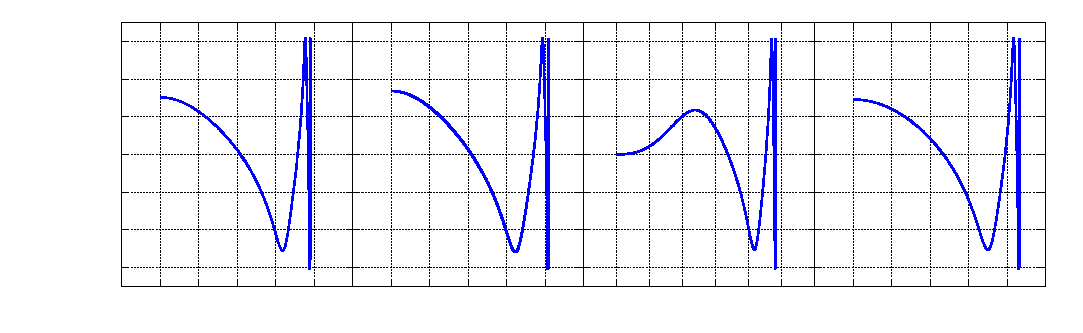
\includegraphics{resources/accumulation_tau_combined}}%
    \gplfronttext
  \end{picture}%
\endgroup
